\section{Localização}

	Calcular a distância de vários pontos na cena relativa a posição da camêra é uma importante tarefa de sistemas de computação visual~\cite{jain}. Para isso, deve-se obter informações de profundidade dos objetos em interesse. Essas informações podem ser obitidas utilizando imagens de itensidade ou de profundidade.

	Uma maneira comum de se obter informações de profundidade de imagens de itensidade é adquirir um par de imagens usando duas câmeras deslocadas entre si por uma distância conhecida. Como alternativa, duas ou mais imagens obtidas de uma camêra em movimento também pode ser utilizadas para calcular informações de profundidade~\cite{jain}.

	Informações 3D também podem ser obitidas indiretamente através de imagens de intensidade utilizando sinais na imagem, como sombreamento e textura~\cite{jain}.

	\begin{figure}[hbt]
		\begin{center}
			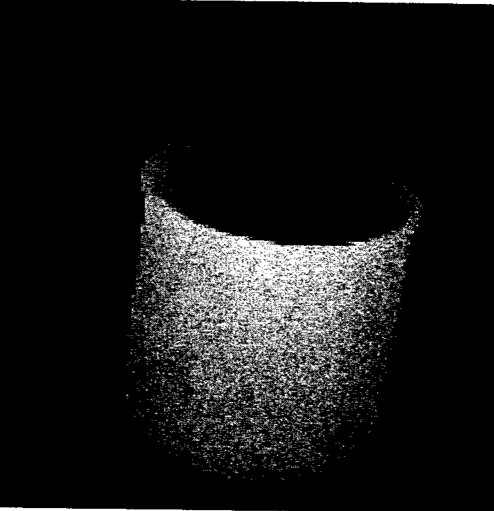
\includegraphics[scale=0.5]{figuras/2.FundamentacaoTeorica/depthimage.png}
		\end{center}
		\caption{Imagem de profundidade de uma caneca de café~\cite{jain}.}
		\label{depthimage}
	\end{figure}

	Em contraste com imagens de itensidade, imagens cujo valor em cada pixel é uma função da distância do ponto correspondente na cena do sensor são chamadas de imagens de pronfunidade, exemplificada na Figura \ref{depthimage}. Tais imagens pode ser adiquiras diretamente utilizando sensores específicos. Os dois métodos mais comuns para obter imagens de profundidade são~\cite{jain}:

		\begin{enumerate}
			\item \textbf{Radar:} a distância até o objeto é calculado observando a diferença de tempo entre o pulso eletromagnético transmitido e recebido. A informação de profundidade também pode ser obtida através da dectecção da diferença de fase entre as ondas trasnsmitidas e as recebidas de um feixe de amplitude modulada~\cite{jain};
			\item \textbf{Triangulação:} utiliza as propriedades geométricas do triângulo para calcular a localização de objetos. Pode ser dividido em duas subcategorias: \textit{lateration} e angulação. \textit{Lateration} computa a posição de um objeto estimando sua distância de múltiplos ponto de referência. Calcular a posição de um objeto em duas dimensões requer estimativas de distância de três pontos não colineares como mostrado na Figura \ref{lateration}. Já em três dimensões são necessários quatro pontos não coplanares. Ângulação utiliza ângulos para determinar a distância do objeto. Em geral, ângulação em duas dimensões requer estimativas de dois ângulos e a estimativa da distância entre dois pontos de referência como mostrado na Figura \ref{angulation}~\cite{triangulacao};
		\end{enumerate}

		\begin{figure}[hbt]
		\begin{center}
			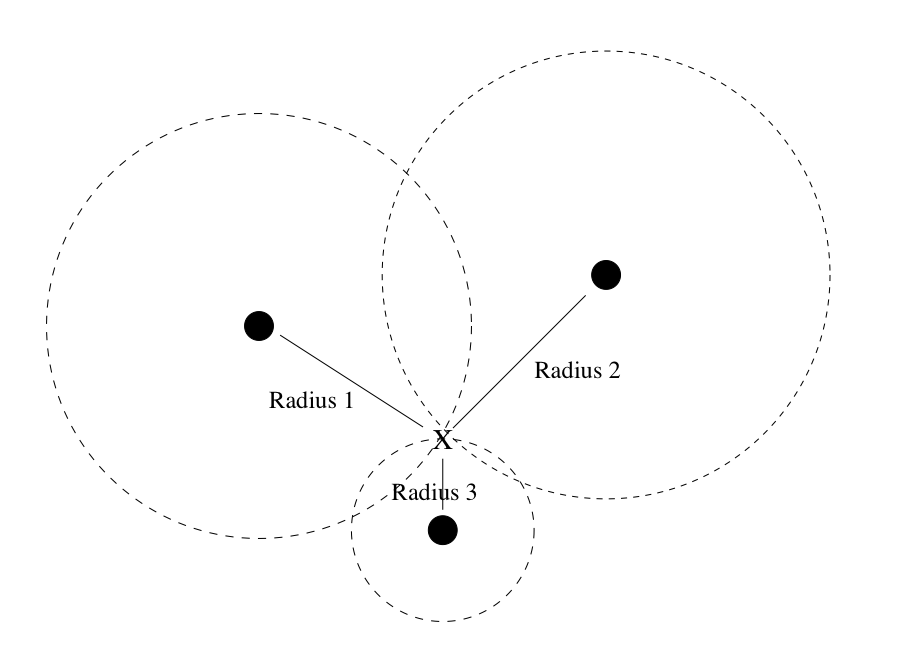
\includegraphics[scale=0.5]{figuras/2.FundamentacaoTeorica/lateration.png}
		\end{center}
		\caption{Determina a distância em duas dimensões utilizando \textit{lateration}. Requer a distância entre o objeto $\displaystyle X$ e três pontos de referência não colineares~\cite{triangulacao}.}
		\label{lateration}
	\end{figure}

	\begin{figure}[hbt]
		\begin{center}
			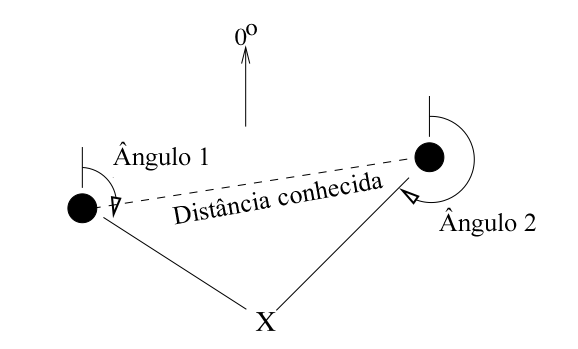
\includegraphics[scale=0.5]{figuras/2.FundamentacaoTeorica/angulation.png}
		\end{center}
		\caption{Exemplo de uma angulação em duas dimensões em que se localiza o objeto $\displaystyle X$ utilizando ângulos relativos a um vetor de referência $\displaystyle 0º$ e a distância entre dois pontos de referência~\cite{triangulacao}.}
		\label{angulation}
	\end{figure}


	Imagens de profundidade são úteis devido a sua especificação explícita de valores de profundidade. Ao mesmo tempo acreditava-se que se a informação de profundidade fosse disponobilizada de maneira explícita, o processamento posterior da imagem seria facilitado. Tournou-se claro que a informação de profundiade ajuda, porém a tarefa básica de interpretação de imagens mantém todas as suas dificuldades~\cite{jain}.

